En esta sección se analizan los resultados obtenidos de las ejecuciones de los algoritmos discutidos en la sección de desarrollo sobre las consultas realizadas en la base de datos de artículos y de las atracciones turísticas. El análisis que se realiza es comparando la calidad de los resultados y el tiempo de ejecución de cada implementación en diferentes condiciones.\\
Para optimizar el tiempo de consulta de la similitud entre dos objetos, se tiene en memoria una matriz con todos los valores de la función similitud. En consecuencia aumenta la complejidad espacial, en las consultas que se realizaron en este trabajo la instancia utilizada no contiene más de $7000$ elementos por lo que la matriz de similitud no supera los $2$ GB de memoria. Por lo tanto, en este caso, es favorable utilizar la matriz.\\

\section{Base de datos de artículos}
De los algorimos descriptos en la sección Desarrollo se ejecutaron pruebas con \texttt{PAC} y \texttt{Búsqueda Golosa}. Con el algoritmo \texttt{PAC} en la etapa de generación de bundles se utilizaron las estrategias \texttt{BOBO-k} y \texttt{Efficient C-HAC} y en la etapa de selección las heurísticas \texttt{Selección de bundles} y \texttt{Selección de bundles proporcional}. Una vez obtenida la solución se aplicaron las búsquedas Tabú para intentar mejorar la solución. En \texttt{PAC} se realiza la búsqueda tabú \texttt{Inter-Bundle} luego de la etapa de producción y la \texttt{Intra-Bundle} luego de la selección. En la \texttt{Búsqueda Golosa} de la solución obtenida se realiza la búsqueda tabú \texttt{Intra-Bundle}.\\

\Solucion
{}
{
\begin{description}
	\item[alg\_1] \texttt{Búsqueda Golosa}
	\item[alg\_2] \texttt{PAC(BOBO-100/Selección de bundles proporcional)}
	\item[alg\_3] \texttt{PAC(BOBO-100/Selección de bundles)}
	\item[alg\_4] \texttt{PAC(Efficient C-HAC/Selección de bundles proporcional)}
	\item[alg\_5] \texttt{PAC(Efficient C-HAC/Selección de bundles)}
\end{description}
}
{$(0,1; 0,3; 0,5; 0,7; 0,9)$}
{10}
{5}
Para comprender el comportamiento de los resultados de las búsquedas se diseñaron dos tipos de gráficos que permiten visualizar de la solución la cohesión de los bundles y la distancia entre ellos. De esta forma se podrá analizar la calidad del resultado obtenido más allá del valor de la función objetivo.\\
Los gráficos del estilo de \ref{res:img-explain-bars} permiten concluir la distribución de los tópicos de una solución a nivel de bundle y de la relación con otros. En los que se visualiza a través del tamaño del círculo la proporción del artículo con el tópico y el color hace referencia al bundle al que el artículo pertenece. Por lo tanto si para un bundle se tiene que la distribución entre los tópicos y el tamaño de los círculos es similar para cada artículo se puede deducir que ese bundle es cohesivo. Por otro lado si el tamaño de los círculos de un bundle no coinciden con los de otro bundle indica que el resultado es diverso.
\begin{figure}[H]
  \centering
    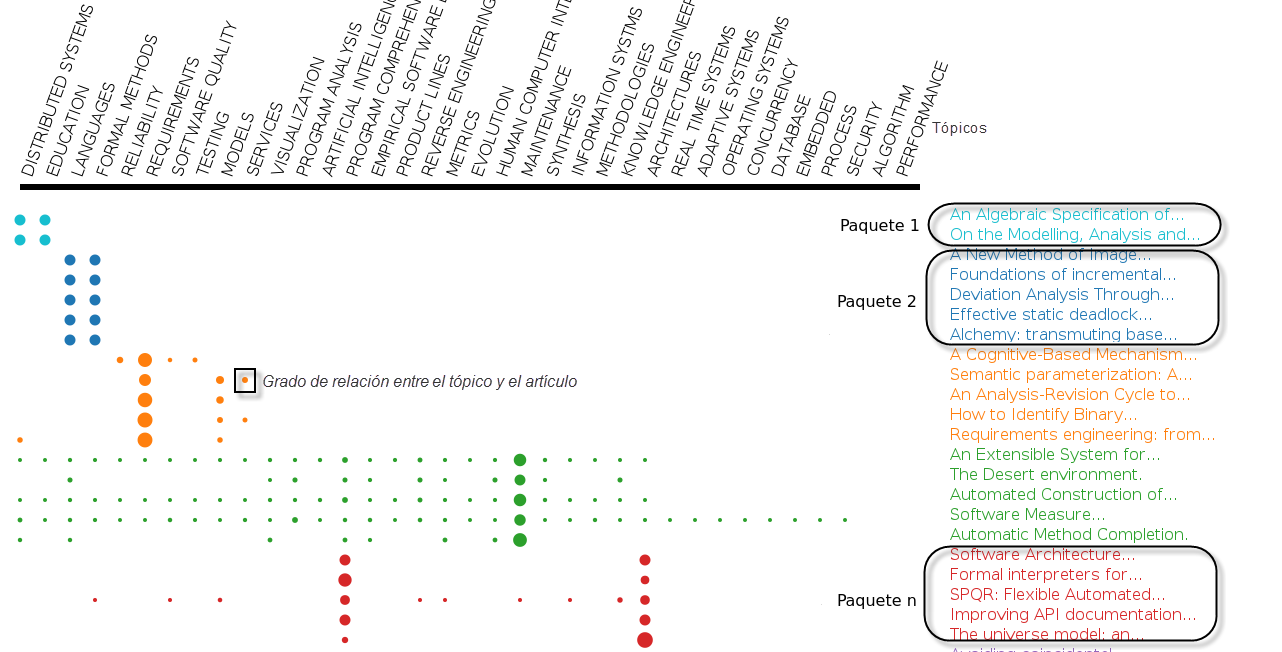
\includegraphics[width=1\textwidth]{img/explain-bars.png}
  \caption{}
  \label{res:img-explain-bars}
\end{figure}

Los gráficos de tipo burbuja \ref{res:img-explain-bubbles} son utiles para concluir el nivel de acoplamiento entre los bundles de una solución, observando la relación entre los tópicos y los bundles. Cada burbuja representa un tópico que contiene círculos; cada circulo es un artículo donde el tamaño es la proporción del articulo con el tópico y el color el bundle al que pertenece. Entonces si las burbujas contienen círculos de más de un color se puede decir que ese resultado no es muy diverso, mientras que el color de los círculos de las burbujas sea más homogéneo el resultado es más diverso. En cuanto a la cohesión de los bundles, es más cohesivo cuando el tamaño de cada circulo dentro de cada burbuja sea similar (para el mismo color) y la distribución de los círculos entre cada burbuja es equitativa.

\begin{figure}[H]
  \centering
    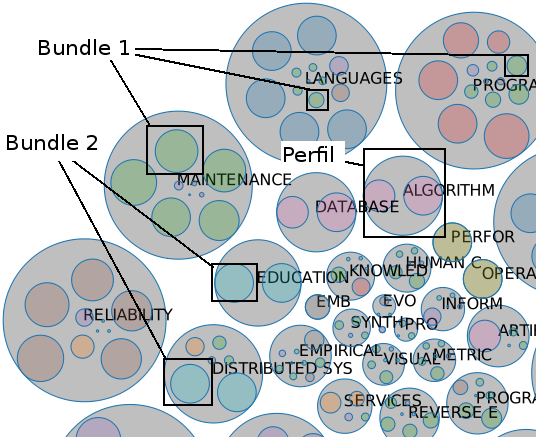
\includegraphics[width=0.5\textwidth]{img/explain-bubbles.png}
  \caption{}
  \label{res:img-explain-bubbles}
\end{figure}



\subsection{Búsquedas de Artículos}\label{res:busPaper}
Generar una solución, en el que cada bundle contenga artículos con tópicos similares que se hayan presentado en distintas conferencias.\\
\begin{itemize}
  \item \textbf{Similitud}: Función que compara el perfil de cada artículo.
  \item \textbf{Complementariedad}: Lugar dónde fue presentado.
\end{itemize}

A partir de las primeras ejecuciones y resultados obtenidos se observaron dos comportamientos no deseados, \textit{soluciones similares para distintos valores de $\gamma$} y \textit{soluciones con bundles unitarios}, a continuación se explica con más detalle estos comportamientos.\\
Al finalizar la depuración de artículos que se consideró afectaban los resultados obtenidos, se obtuvieron $3954$ para realizar todas las pruebas mencionadas.
\paragraph{Soluciones similares para distintos gammas}
En las primeras ejecuciones realizada se observa que el valor de la función objetivo se encuentra cercano a una cota máxima (ver \ref{conc:valoresOptimos}) y que para todos los valores de $\gamma$ utilizados las soluciones eran muy similares entre sí. Realizando un análisis más detallado sobre los resultados se detectó que la mayoría de los bundles contenían artículos de un solo tópico, o sea bundles  muy cohesivo internamente(alto valor \textbf{intra}) y muy diversos entre si (alto valor \textbf{inter}).\\
Al contar con muchos artículos con un solo tópico las soluciones obtenidas no permiten realizar una correcta comparación de las heurísticas, por lo tanto a fines prácticos de comparar las distintas implementaciones y obtener un conjunto de bundles más interesantes, se decidió eliminar los artículos que contengan un solo un tópico.
\paragraph{Soluciones con bundles unitarios}
Las soluciones obtenidas mediante las búsquedas en las que se prioriza que los bundles sean más cohesivos (\textbf{inter}) contenían una alta cantidad de bundles con uno o dos elementos únicamente, tal conducta no es la deseada ya que queda una parte del presupuesto sin ser usado.\\
Este comportamiento ocurre particularmente con el método jerárquico o HAC en la etapa de producción del algoritmo \texttt{PAC}, ya que algunos cluster generados no superan el presupuesto pero no pueden ser unidos con otro cluster porque invalida la complementariedad que se quiere lograr. Suponiendo que para la búsqueda \textit{Artículos de diferentes conferencias} existen los artículos $A_1$, $A_2$, $A_3$, $A_4$ y $A_5$ y tienen una distribución del tópico $t$ mayor a $0.7$, es lógico que se genere un bundle con estos 5 artículos porque es cohesivo. Ahora si las conferencias son $V_1, V_2$ y $V_3$ y los artículos se presentan de la siguiente manera:
\begin{itemize}
	\item $A_1$ $\rightarrow$ $V_1$
	\item $A_2$ $\rightarrow$ $V_2$
	\item $A_3,\ A_4\ y\ A_5$ $\rightarrow$ $V_3$
\end{itemize} 

Entonces para el criterio de búsqueda los artículos $A_3, A_4$ y $A_5$ no pueden pertenecer al mismo bundle pues éstos no son complementarios entre sí.\\
El proceso de clusterización jerárquico, puede generar la siguiente configuración en la cual no se pueden unir los bundles, el bundle $B_1$ con los artículos $A_1$ y $A_3$ el bundle $B_2$ con los artículos $A_2$ y $A_4$ y el bundle $B_3$ con el artículo $A_5$. Efectivamente esta clusterización no es óptima para el problema porque se podría haber generado un bundle más cohesivo (\textbf{mayor intra}) si se hubiera elegido el siguiente bundle $A_1$, $A_2$ y $A_3$.\\
La propuesta para corregir esta situación fue la de realizar una Búsqueda Tabú al finalizar la etapa del \textit{Produce} con los bundles ya generados así de esta forma mejorar el intra de los bundles antes de la etapa de selección.

\newpage

En los gráficos \ref{res:img-papers-agr-gamma01} y \ref{res:img-papers-agr-gamma09} se muestran agrupados por algoritmo de resolución las diferentes estrategias usadas en cada caso y los valores de la función objetivo alcanzado toma los dos extremos del valor de $\gamma$ $0.1$ y $0.9$. 

\begin{figure}[H]
  \centering
    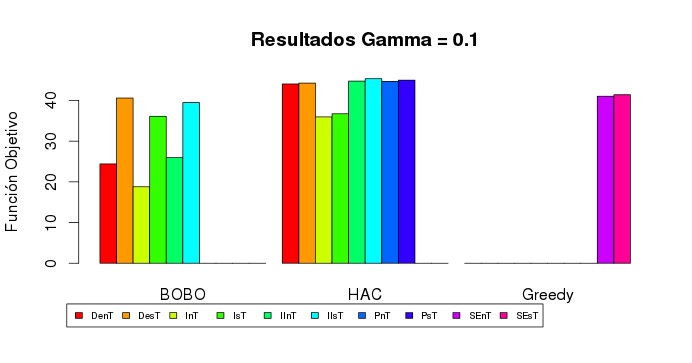
\includegraphics[width=0.8\textwidth]{resultados/papers/Graficos_agrupados/gamma01.png}
  \caption{Función Objetivo $\gamma$ = $0.1$ vs Algoritmos de resolución}
  \label{res:img-papers-agr-gamma01}
\end{figure}

\begin{figure}[H]
  \centering
    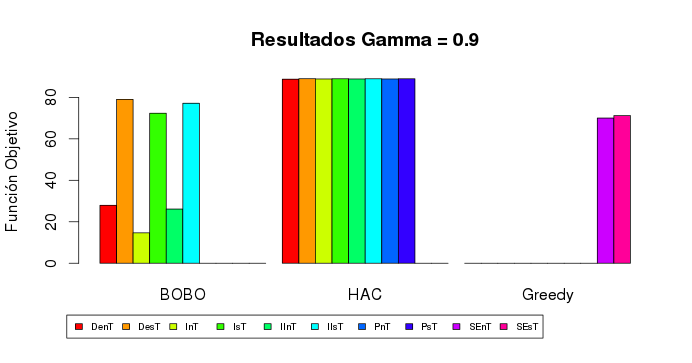
\includegraphics[width=0.8\textwidth]{resultados/papers/Graficos_agrupados/gamma09.png}
  \caption{Función Objetivo $\gamma$ = $0.9$ vs Algoritmos de resolución}
  \label{res:img-papers-agr-gamma09}
\end{figure}

De lo anterior se observa que para todos valores de $\gamma$ las soluciones obtenidas al aplicar la búsqueda tabú se mejora la función objetivo, en el caso de BOBO la mejora es más significativa que en los otros.\\

\paragraph{Jerárquico (Efficient C-HAC)}
En \ref{res:img-papers-agr-gamma01} y \ref{res:img-papers-agr-gamma09} se visualiza que utilizando la búsqueda Tabú al final de la ejecución de HAC no mejora considerablemente la solución. Por lo que se decidió para este caso comparar el algoritmo sin la búsqueda tabú.
\begin{figure}[H]
  \centering
    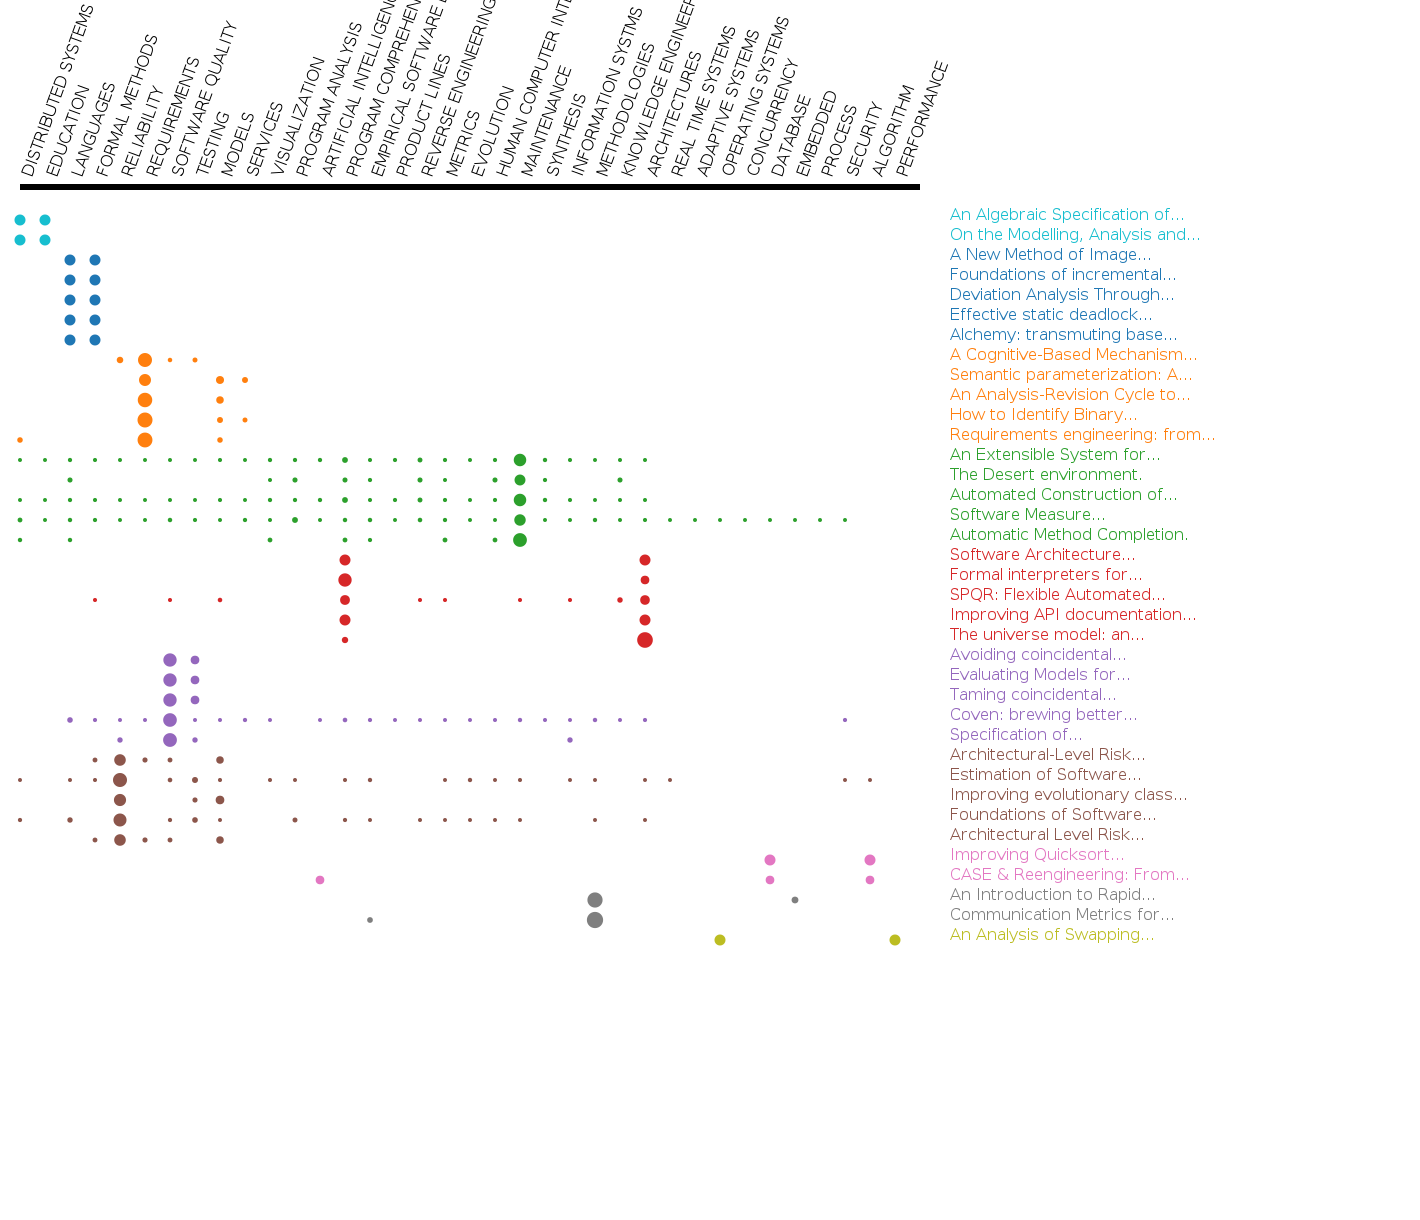
\includegraphics[width=0.8\textwidth]{resultados/papers/HAC/INTRA_INTER/gamma-01.png}
  \caption{Distribución de los perfiles por artículo y bundle $\gamma$ = $0.1$ y HAC - Intra Inter}
  \label{res:img-papers-gamma01-hac-intra-inter}
\end{figure}

\begin{figure}[H]
  \centering
    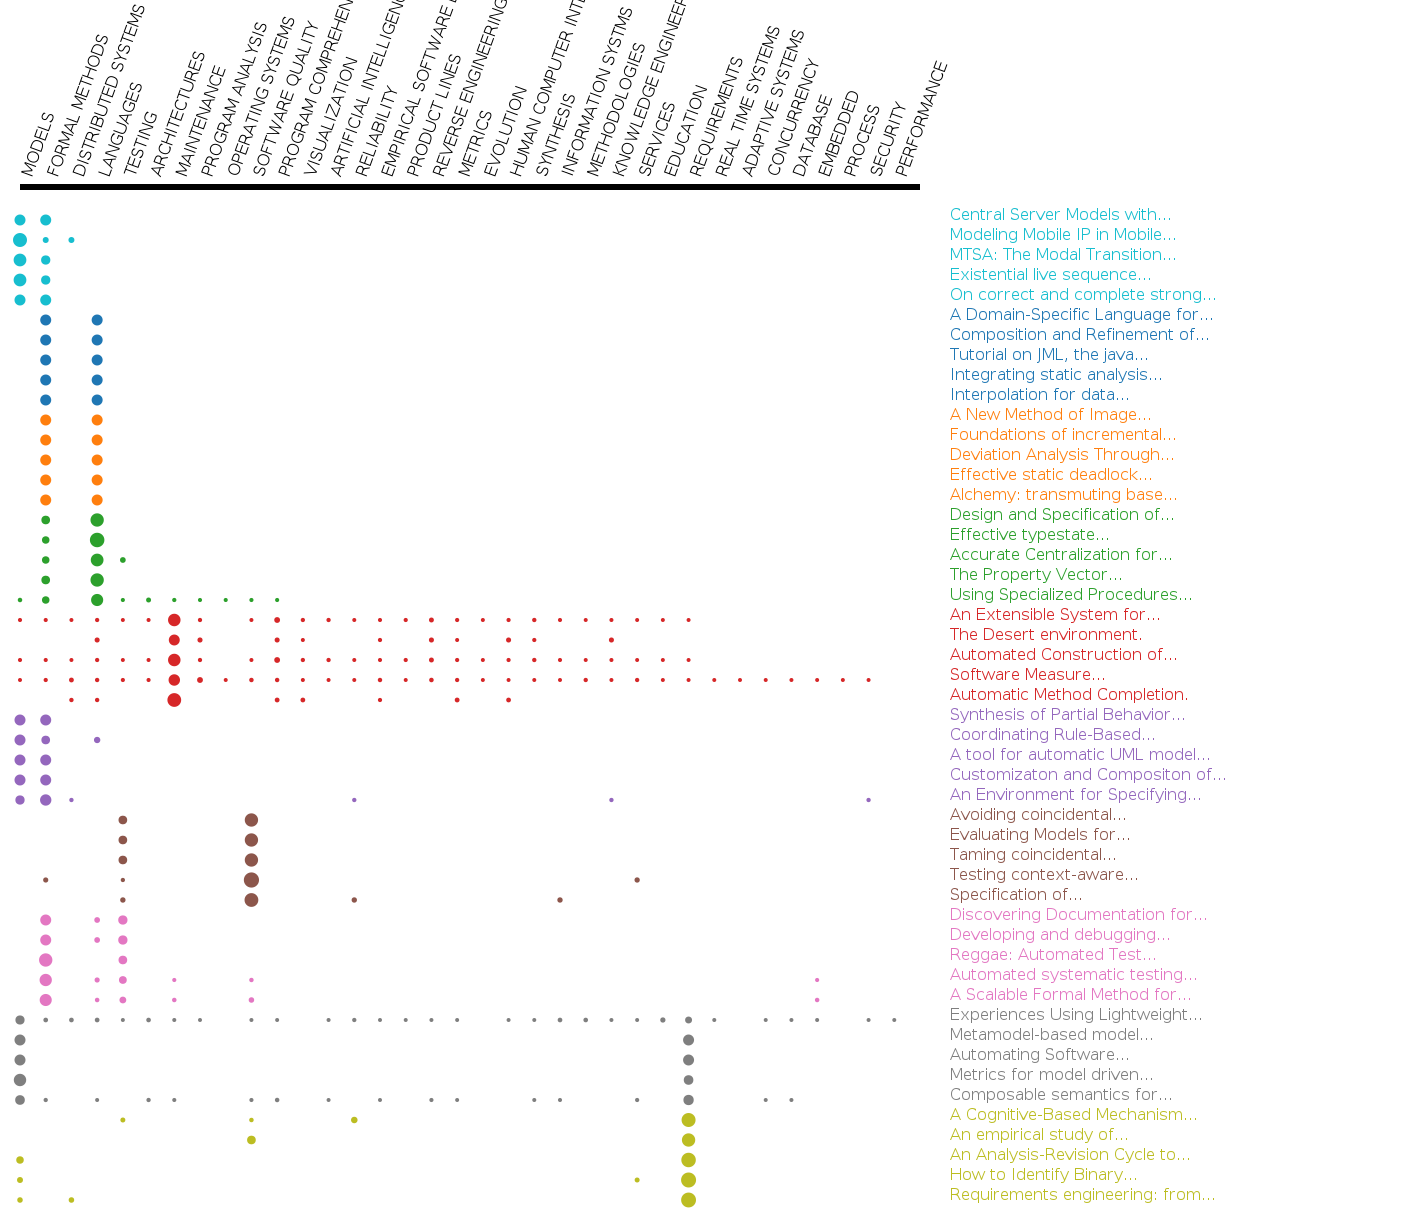
\includegraphics[width=0.8\textwidth]{resultados/papers/HAC/INTRA_INTER/gamma-09.png}
  \caption{Distribución de los perfiles por artículo y bundle $\gamma$ = $0.9$ y HAC - Intra Inter}
  \label{res:img-papers-gamma09-hac-intra-inter}
\end{figure}

\begin{figure}[H]
  \centering
    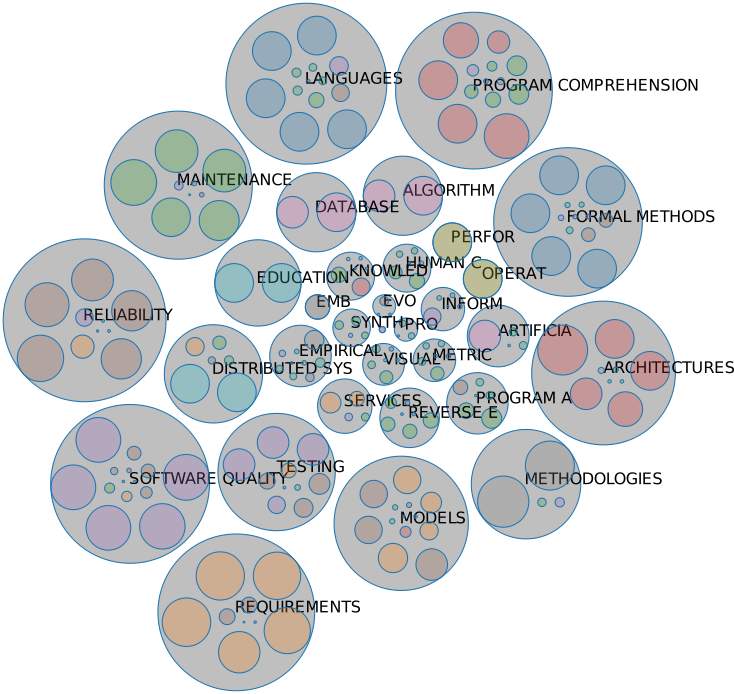
\includegraphics[width=0.8\textwidth]{resultados/papers/HAC/INTRA_INTER/bubbles-gamma-01.png}
  \caption{Distribución de los artículos por perfil $\gamma$ = $0.1$ y HAC - Intra Inter}
  \label{res:img-papers-bubbles-gamma01-hac-intra-inter}
\end{figure}

\begin{figure}[H]
  \centering
    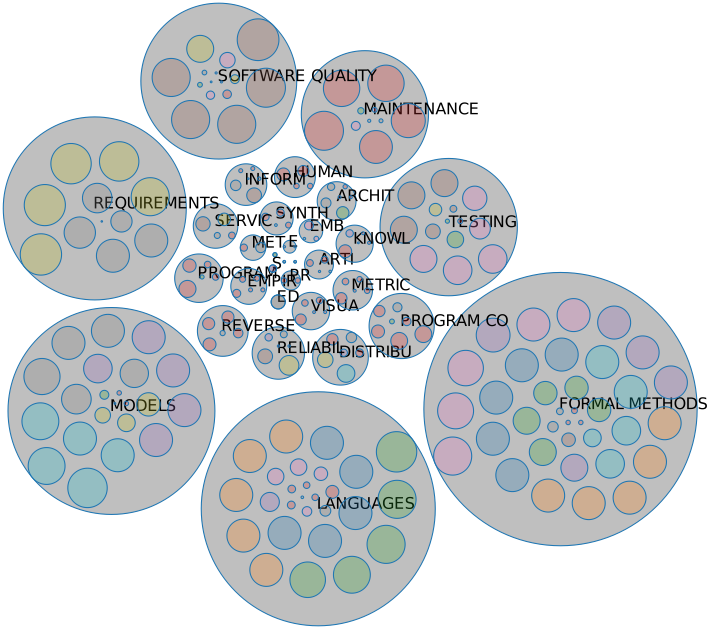
\includegraphics[width=0.8\textwidth]{resultados/papers/HAC/INTRA_INTER/bubbles-gamma-09.png}
  \caption{Distribución de los papers por perfil $\gamma$ = $0.9$ y HAC - Intra Inter}
  \label{res:img-papers-bubbles-gamma09-hac-intra-inter}
\end{figure}

De los gráficos \ref{res:img-papers-gamma01-hac-intra-inter} y \ref{res:img-papers-gamma09-hac-intra-inter} se observa que para $\gamma$ con valor cercano a cero, la solución contiene artículos con perfiles que cubren varios tópicos mientras que para $\gamma$ con valores más cercanos a uno, los tópicos de los artículos se concentran en unos pocos. Con esto se cumple el requerimiento de que cuando $\gamma$ se acerca el bundle es más cohesivo pero menos diverso (en \ref{res:img-papers-bubbles-gamma09-hac-intra-inter}. se observa la concentración de tópicos que hay en la solución).\\
Este comportamiento se repitió para todas las estrategias de selección que se utilizaron, la única diferencia fueron los valores finales de la función objetivo.
\paragraph{BOBO-100}
En este caso al ser muy grande la diferencia entre la utilización de la heurística Tabú y la ejecución sin ella,  se incluyó la misma para poder visualizar los cambios en la solución.
\begin{figure}[H]
  \centering
    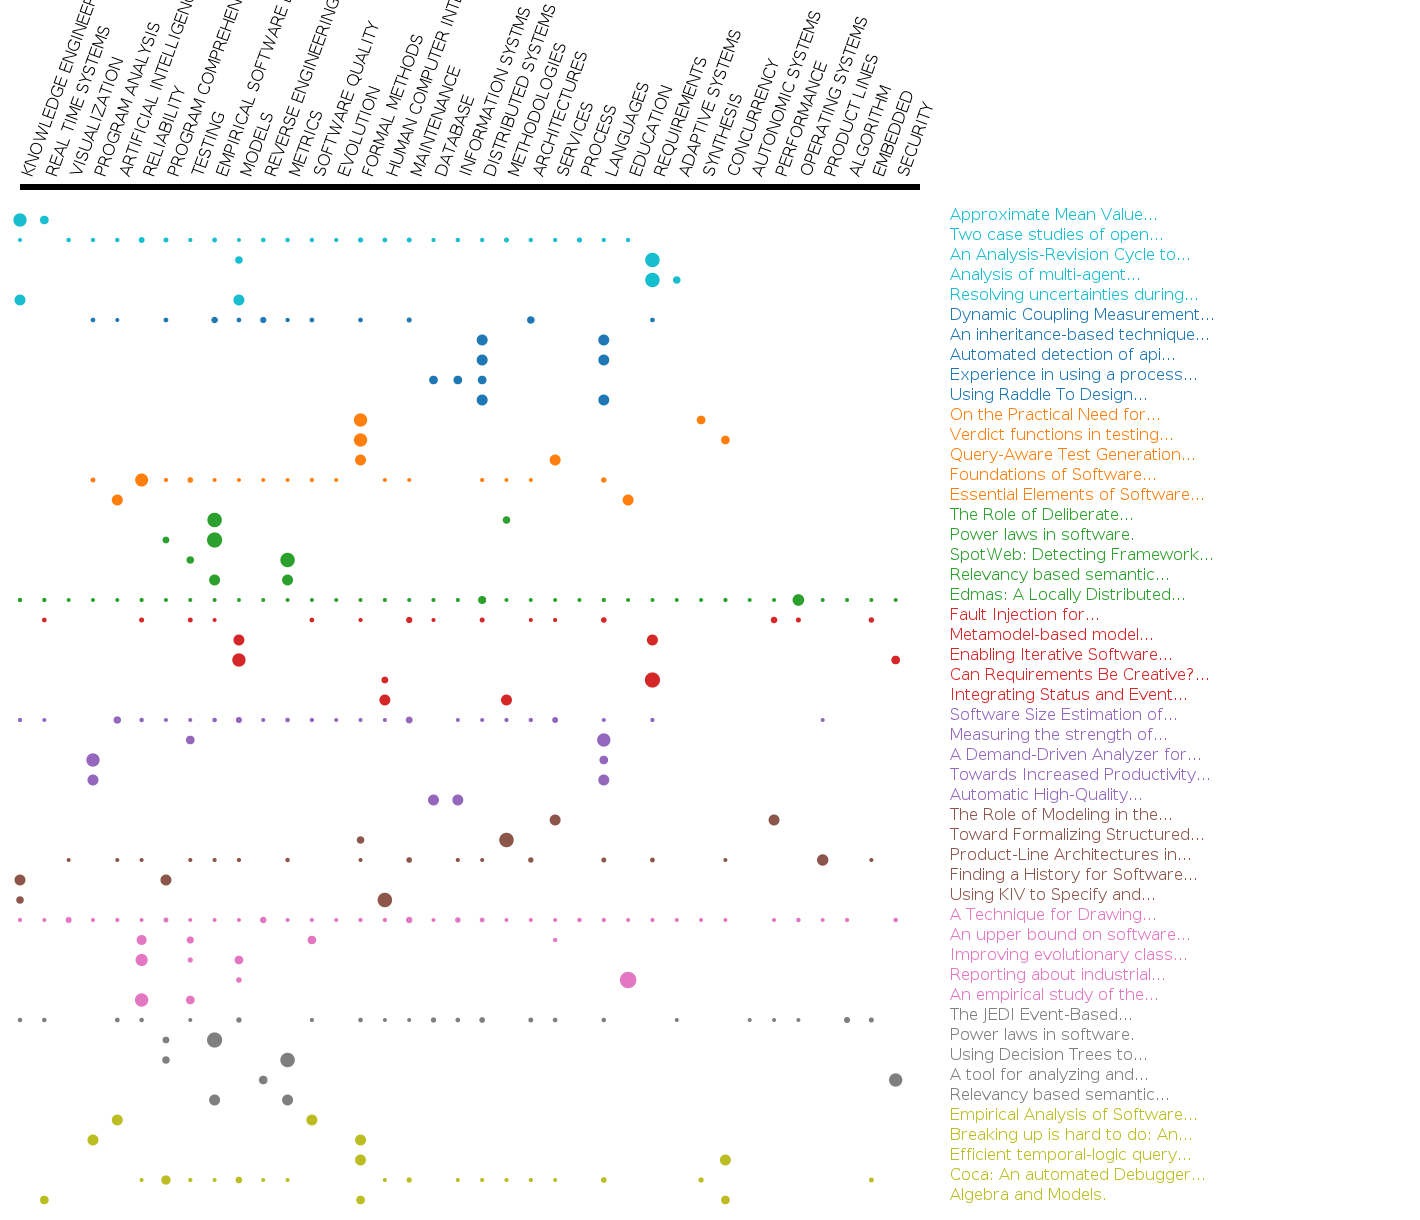
\includegraphics[width=0.8\textwidth]{resultados/papers/BOBO/INTRA_INTER/gamma-01.png}
  \caption{Distribución de los perfiles por artículo y bundle $\gamma$ = $0.1$ y BOBO - Intra Inter}
  \label{res:img-papers-gamma01-bobo-intra-inter}
\end{figure}

\begin{figure}[H]
  \centering
    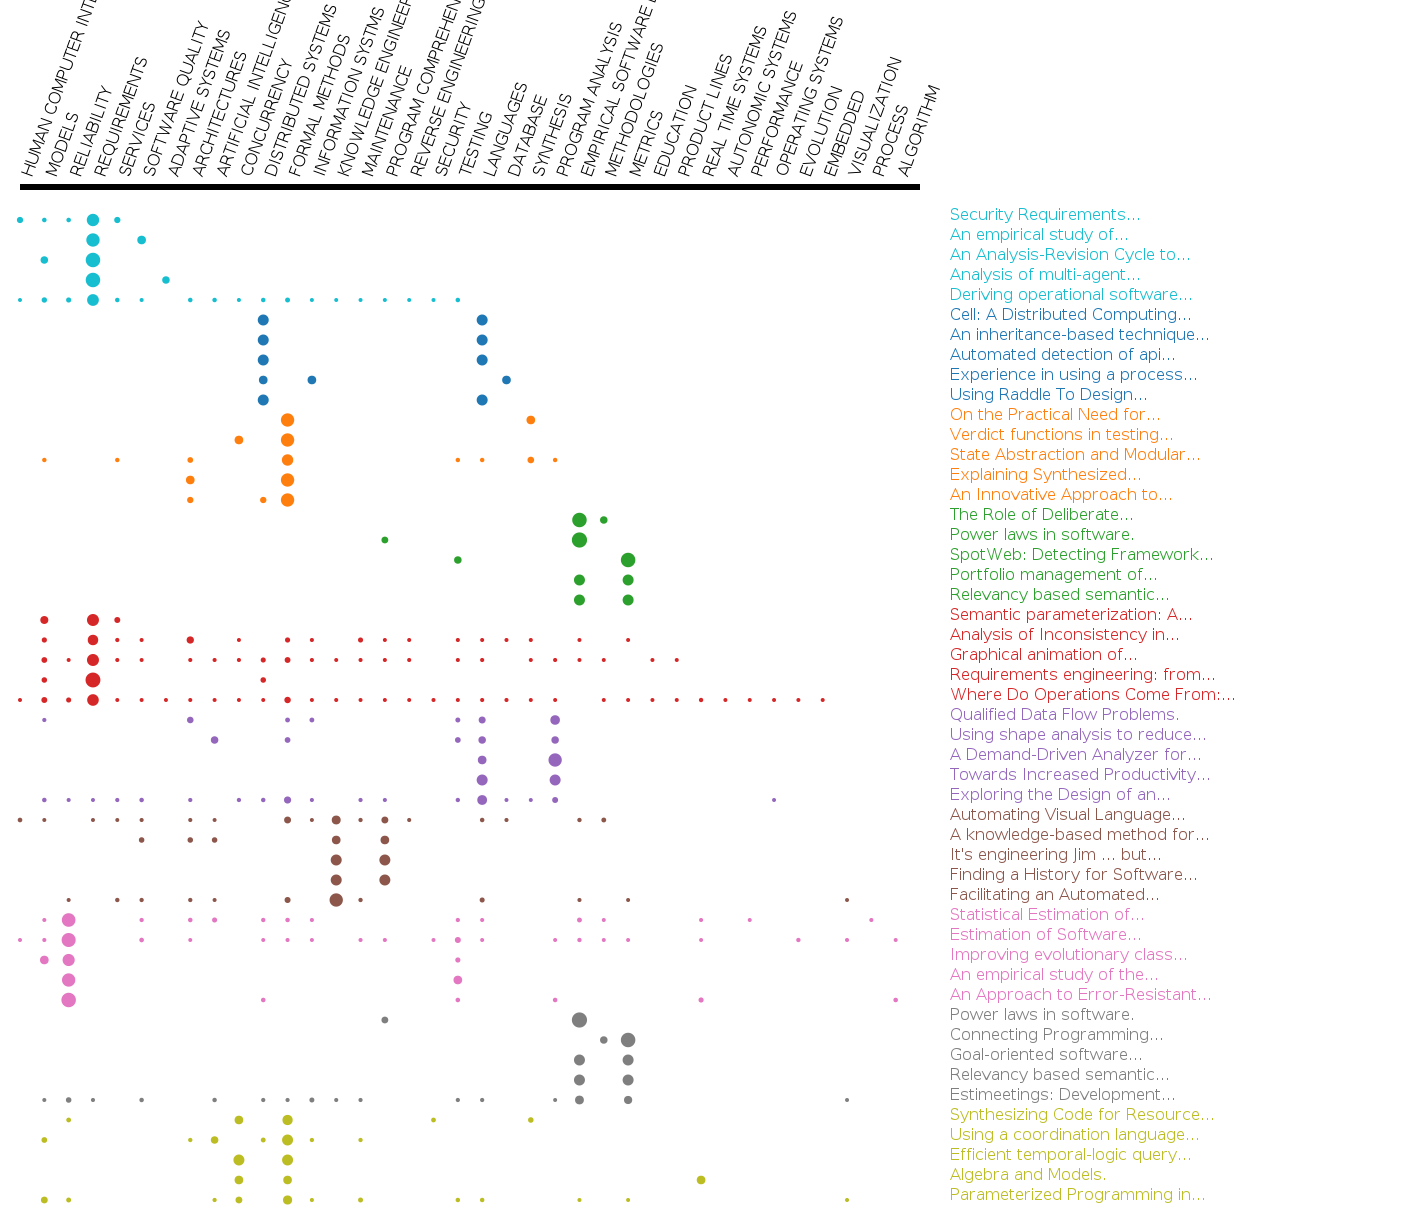
\includegraphics[width=0.8\textwidth]{resultados/papers/BOBO/INTRA_INTER/gamma-with-local-01.png}
  \caption{Distribución de los perfiles por artículo y bundle $\gamma$ = $0.1$ y BOBO - Intra Inter con búsqueda Tabú}
  \label{res:img-papers-gamma01-bobo-intra-inter-tabu}
\end{figure}

\begin{figure}[H]
  \centering
    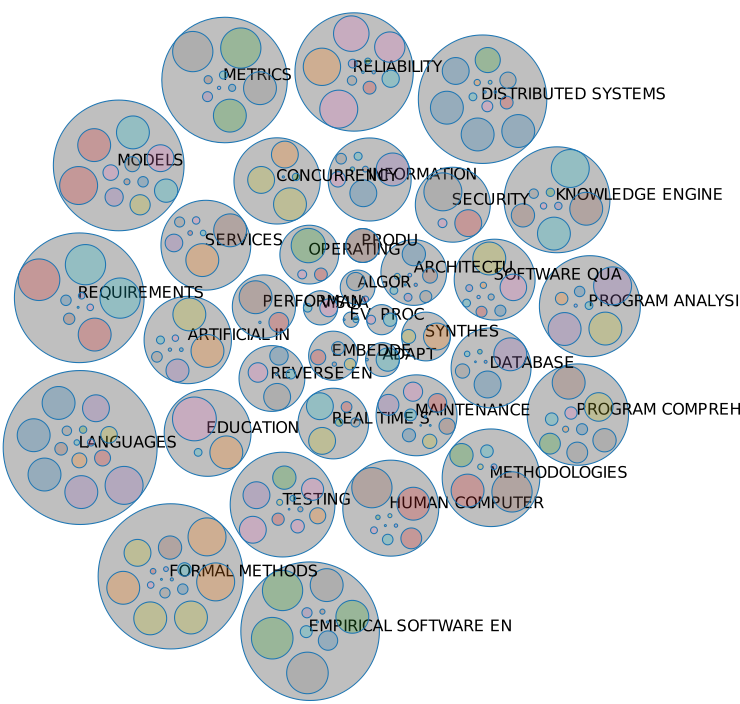
\includegraphics[width=0.8\textwidth]{resultados/papers/BOBO/INTRA_INTER/bubbles-gamma-01.png}
  \caption{Distribución de los artículos por perfil $\gamma$ = $0.1$ y BOBO - Intra Inter}
  \label{res:img-papers-bubbles-gamma01-bobo-intra-inter}
\end{figure}

\begin{figure}[H]
  \centering
    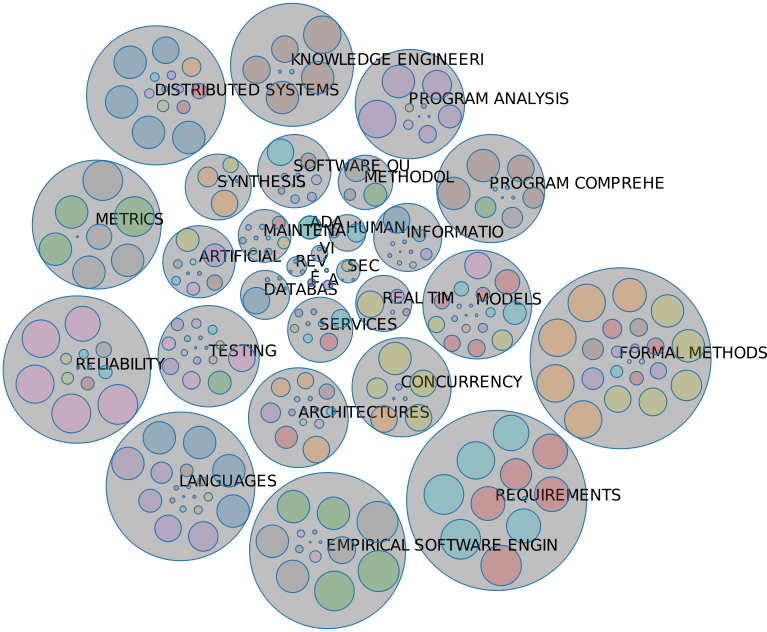
\includegraphics[width=0.8\textwidth]{resultados/papers/BOBO/INTRA_INTER/bubbles-gamma-with-local-01.png}
  \caption{Distribución de los artículos por perfil $\gamma$ = $0.1$ y BOBO - Intra Inter con búsqueda Tabú}
  \label{res:img-papers-bubbles-gamma01-hac-intra-inter-bobo}
\end{figure}

\begin{figure}[H]
  \centering
    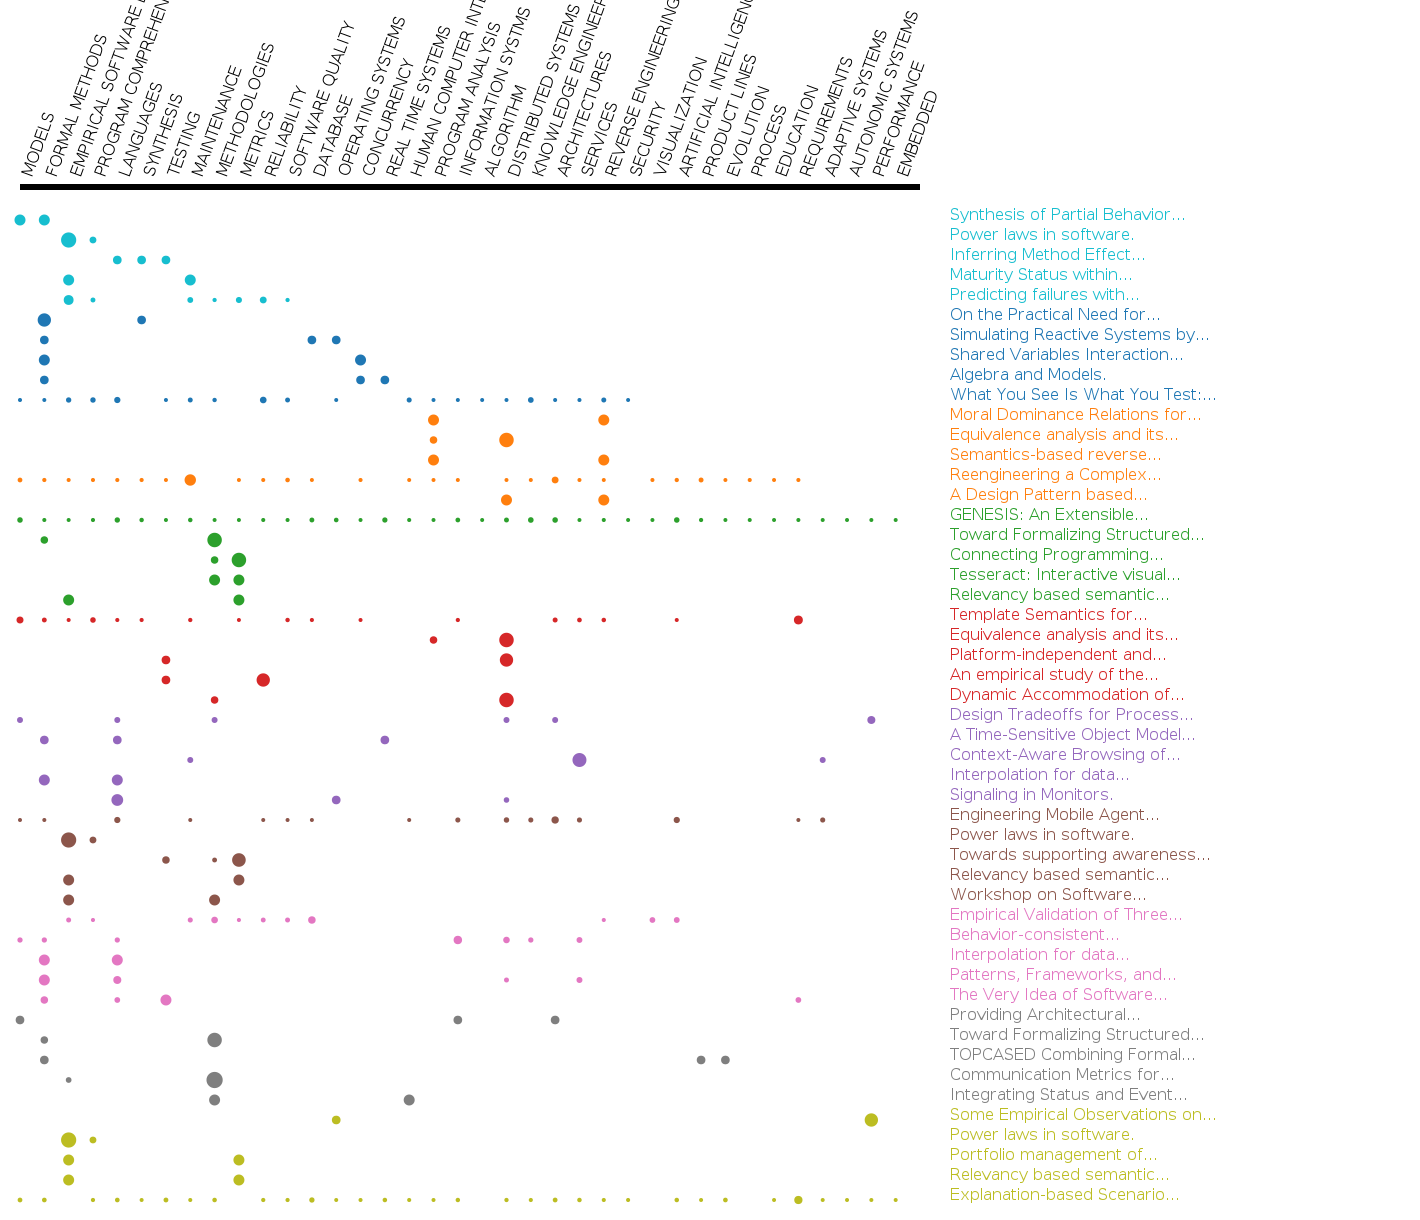
\includegraphics[width=0.8\textwidth]{resultados/papers/BOBO/INTRA_INTER/gamma-09.png}
  \caption{Distribución de los perfiles por artículo y bundle $\gamma$ = $0.9$ y BOBO - Intra Inter}
  \label{res:img-papers-gamma09-bobo-intra-inter}
\end{figure}

\begin{figure}[H]
  \centering
    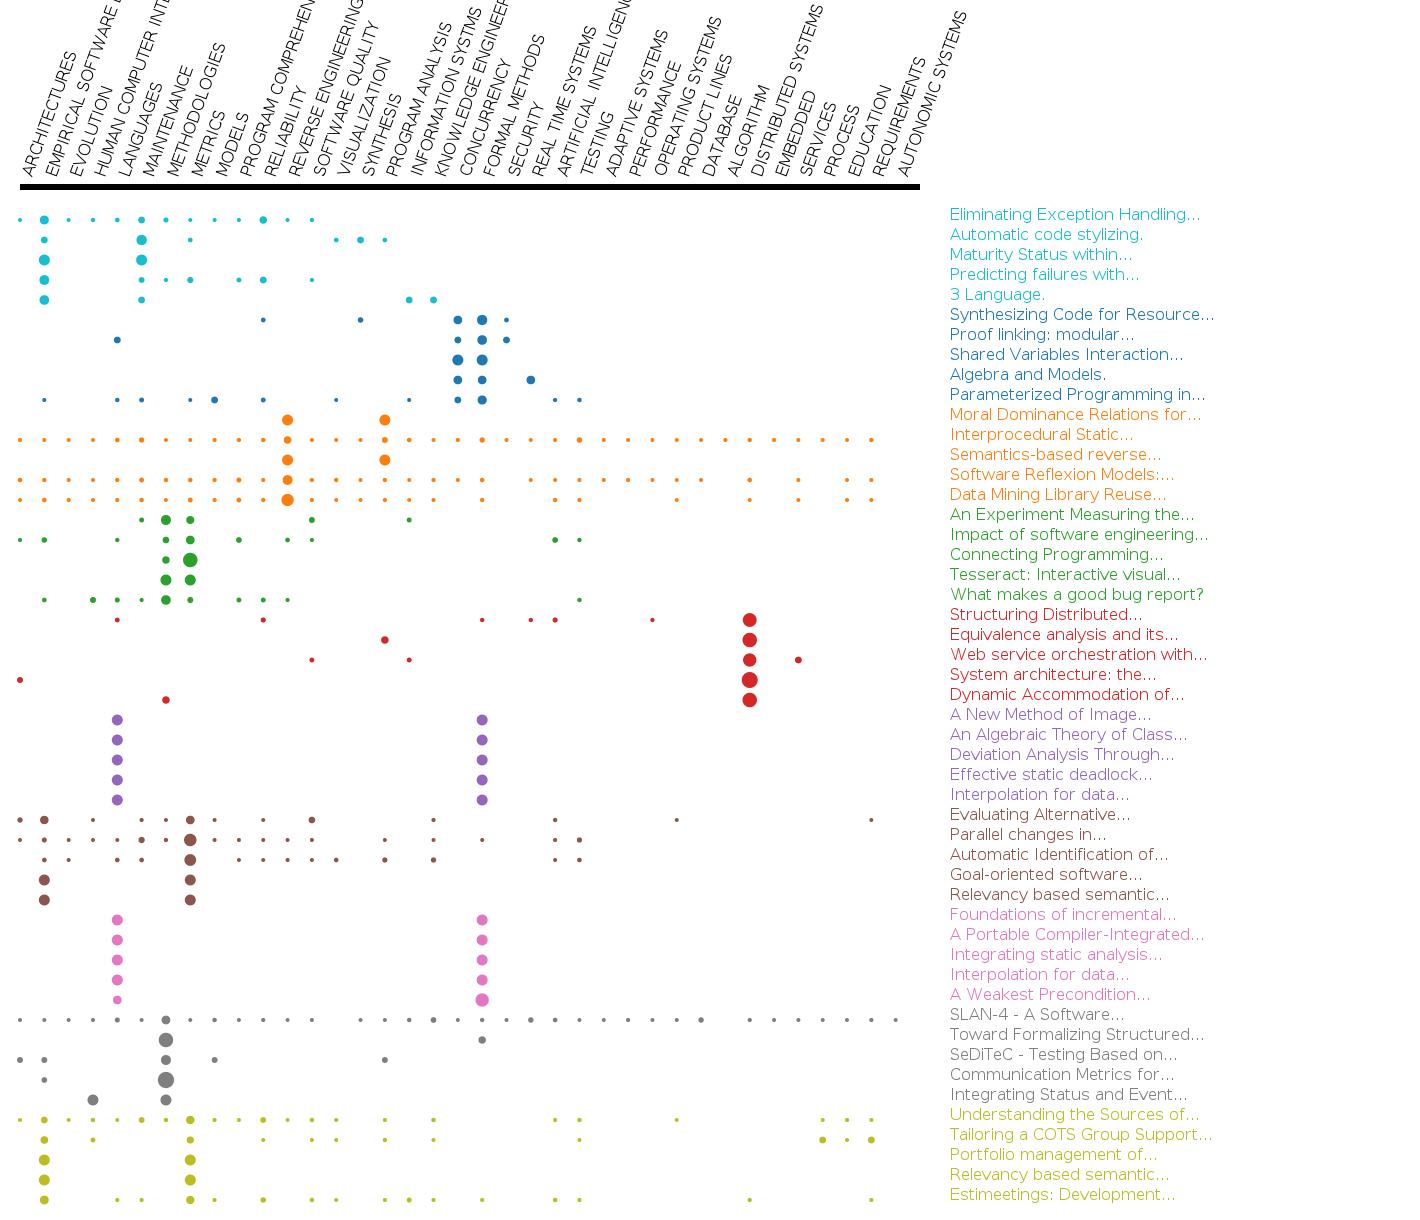
\includegraphics[width=0.8\textwidth]{resultados/papers/BOBO/INTRA_INTER/gamma-with-local-09.png}
  \caption{Distribución de los perfiles por artículo y bundle $\gamma$ = $0.9$ y BOBO - Intra Inter con búsqueda Tabú}
  \label{res:img-papers-gamma09-bobo-intra-inter-tabu}
\end{figure}

\begin{figure}[H]
  \centering
    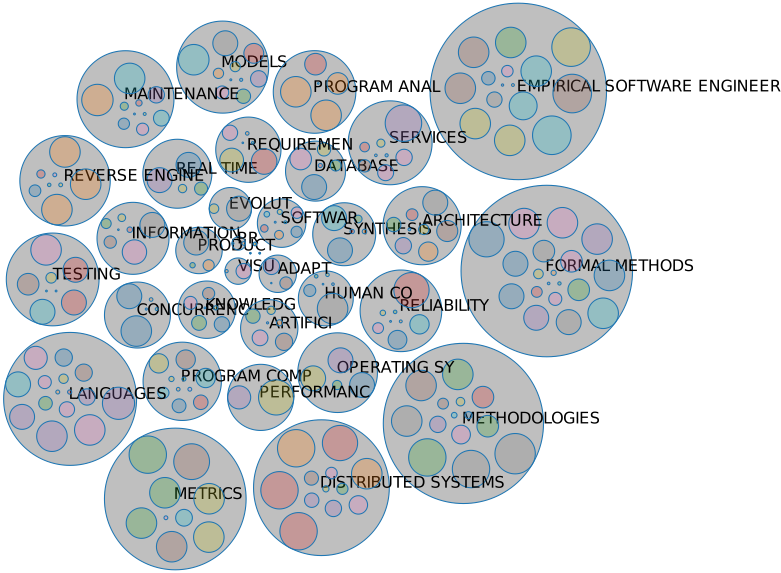
\includegraphics[width=0.8\textwidth]{resultados/papers/BOBO/INTRA_INTER/bubbles-gamma-09.png}
  \caption{Distribución de los artículos por perfil $\gamma$ = $0.9$ y BOBO - Intra Inter}
  \label{res:img-papers-bubbles-gamma09-bobo-intra-inter}
\end{figure}

\begin{figure}[H]
  \centering
    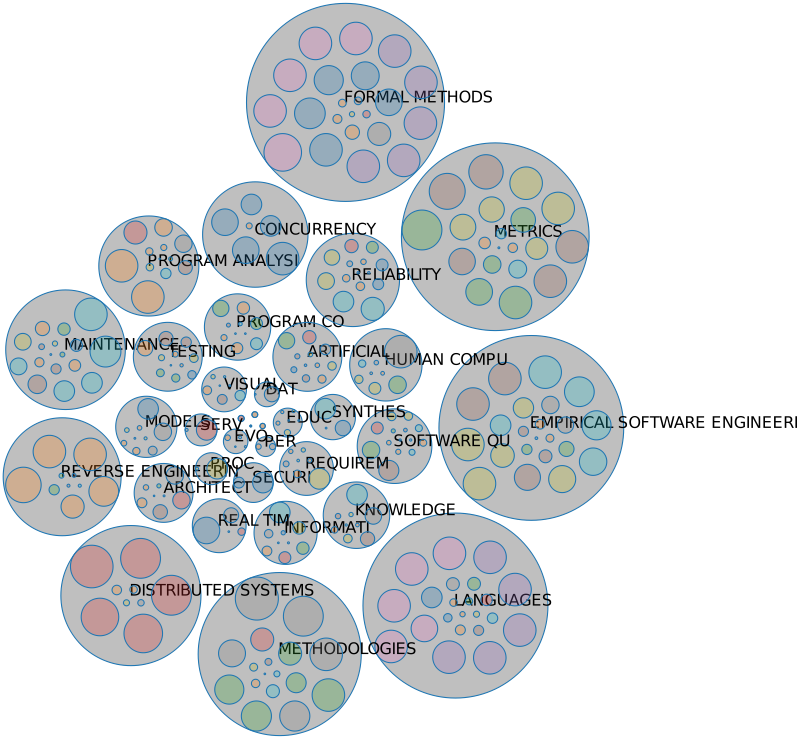
\includegraphics[width=0.8\textwidth]{resultados/papers/BOBO/INTRA_INTER/bubbles-gamma-with-local-09.png}
  \caption{Distribución de los artículos por perfil $\gamma$ = $0.9$ y BOBO - Intra Inter con búsqueda Tabú}
  \label{res:img-papers-bubbles-gamma09-hac-intra-inter-bobo}
\end{figure}
\newpage
\subsection{Búsqueda de Autores}
Solución de bundles en el que cada uno contiene autores que escribieron artículos de tópicos similares y pertenecen a distinta universidad.\\
\begin{itemize}
  \item \textbf{Similitud}: Función que compara el perfil de los autores.
  \item \textbf{Complementariedad}: Universidad de pertenencia del autor.
\end{itemize}

La instancia elegida, luego de la depuración, cuenta con $5577$ autores en condiciones de ser elegidos por los algoritmos implementados.\\

\begin{figure}[H]
  \centering
    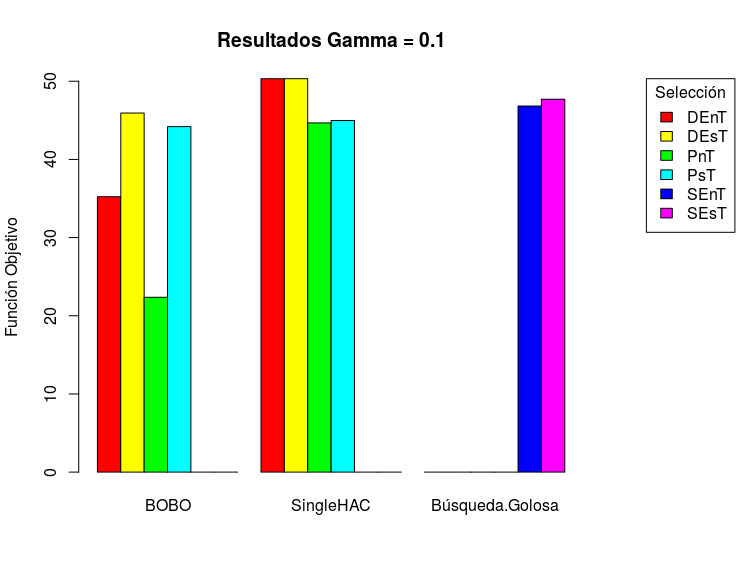
\includegraphics[width=0.8\textwidth]{resultados/authors/Graficos_agrupados/gamma01-autores.png}
  \caption{Función Objetivo $\gamma$ = $0.1$ vs Algoritmos de resolución}
  \label{res:img-autores-agr-gamma01}
\end{figure}

\begin{figure}[H]
  \centering
    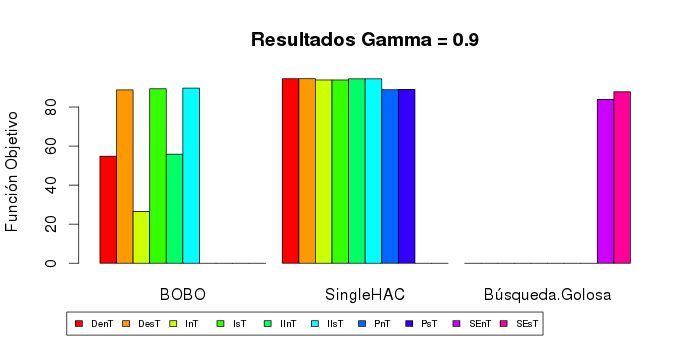
\includegraphics[width=0.8\textwidth]{resultados/authors/Graficos_agrupados/gamma09-autores.png}
  \caption{Función Objetivo $\gamma$ = $0.9$ vs Algoritmos de resolución}
  \label{res:img-autores-agr-gamma09}
\end{figure}

El comportamiento de las ejecuciones fueron muy similares a las que se obtuvieron en la búsqueda de artículos. La utilización de la Búsqueda Tabú mejoró sustancialmente el algoritmo \texttt{BOBO} en todos sus variantes. En el caso de \texttt{SingleHAC}, solo mejoró con la estratégia de selección \texttt{Proportional}. Casualmente fue la única estrategia que tuvo un comportamiento diferente en relación a la búsqueda de artículos, en la cuál la función objetivo siempre tuvo valores mayores o iguales a por ejemplo la selección \texttt{INTRA} y en este caso fue menor o igual. Igualmente las diferencias en términos de valor son mínimas y se deben a la conformación de los perfiles de los elementos.\\
Como se menciona anteriormente, al no comportarse de una manera diferente a la búsqueda de artículos no se incluyeron los gráficos.
\newpage
\subsection{Búsqueda de universidades}\label{res:busInstituciones}
Solución de bundles en el que cada uno contiene universidades de distintas regiones en las que se escribieron artículos de tópicos.\\
\begin{itemize}
  \item \textbf{Similitud}: Función que compara el perfil de las instituciones.
  \item \textbf{Complementariedad}: Región a la que pertence la instituciones.
\end{itemize}

\begin{figure}[H]
  \centering
    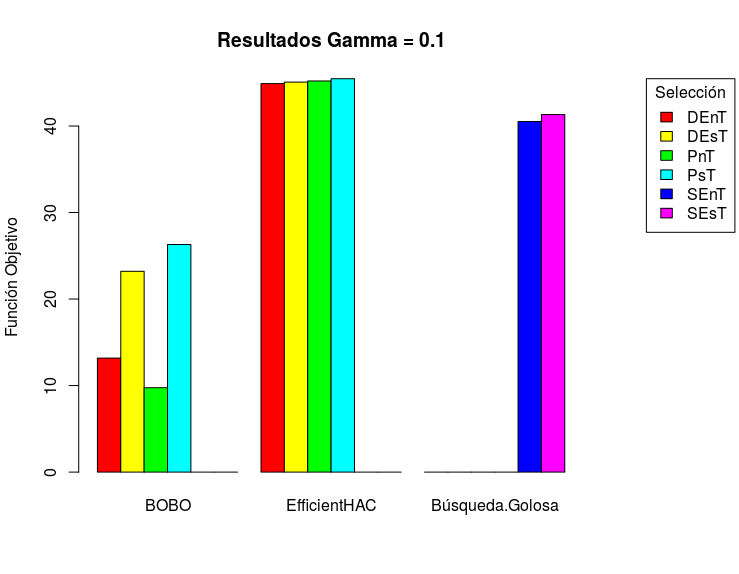
\includegraphics[width=0.8\textwidth]{resultados/affiliations/Graficos_agrupados/gamma01-affiliations.png}
  \caption{Función Objetivo $\gamma$ = $0.1$ vs Algoritmos de resolución}
  \label{res:img-affiliations-agr-gamma01}
\end{figure}

\begin{figure}[H]
  \centering
    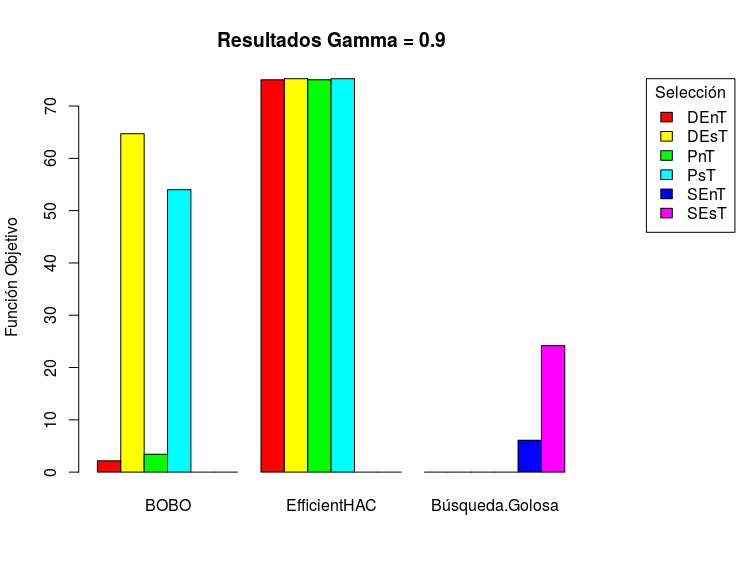
\includegraphics[width=0.8\textwidth]{resultados/affiliations/Graficos_agrupados/gamma09-affiliations.png}
  \caption{Función Objetivo $\gamma$ = $0.9$ vs Algoritmos de resolución}
  \label{res:img-affiliations-agr-gamma09}
\end{figure}

Como se observa en los gráficos anteriores el uso de las búsquedas Tabú siempre mejora la solución obtenida en primer lugar, sin importar que algoritmo se haya utilizado previamente. Particularmente, y al igual que en los demás experimentos, la variante \texttt{BOBO} es siempre la más beneficiada por el uso de la metaheurística ya que el valor de la función objetivo de la solución final por lo menos duplica al correspondiente de la solución original.\\
A difierencia de los escenarios anteriores el algoritmo \texttt{Goloso} para $\gamma\ =\ 0.9$ no obtuvo resultados buenos como se esperaba.
\newpage
\section{Búsqueda de atracciones turísticas}\label{res:busAtracciones}
Aquí se muestran las soluciones en las que cada bundle representa un conjunto de atracciones que un turista puede visitar, cada uno de ellos no supera el presupuesto máximo y cada elemento es un tipo de atracción diferente. resultados
\begin{itemize}
  \item \textbf{Similitud}: Los valores fueron entregados ya calculados.
  \item \textbf{Complementariedad}: Tipo de atracción turística.
  \item \textbf{Presupuesto}: Cantidad de dinero que tiene el usuario para utilizar.
\end{itemize}
Se generaron soluciones con las siguientes características:\\
\SolucionBudget
{}
{
\begin{description}
	\item[alg\_1] \texttt{Búsqueda Golosa}
	\item[alg\_2] \texttt{PAC(BOBO-100/Selección de bundles proporcional)}
	\item[alg\_3] \texttt{PAC(BOBO-100/Selección de bundles)}
	\item[alg\_4] \texttt{PAC(Efficient C-HAC/Selección de bundles proporcional)}
	\item[alg\_5] \texttt{PAC(Efficient C-HAC/Selección de bundles)}
\end{description}
}
{$(0,1; 0,3; 0,5; 0,7; 0,9)$}
{10}
{3}
{7}

\begin{figure}[H]
  \centering
    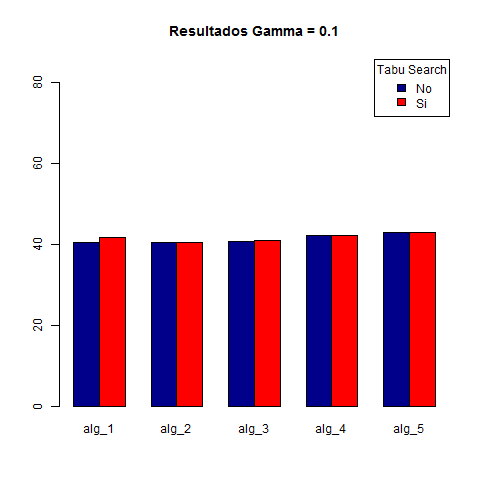
\includegraphics[width=0.8\textwidth]{resultados/cities/Graficos_agrupados/gamma01-cities.png}
  \caption{Función Objetivo $\gamma$ = $0.1$ vs Algoritmos de resolución}
  \label{res:img-cities-agr-gamma01}
\end{figure}

\begin{figure}[H]
  \centering
    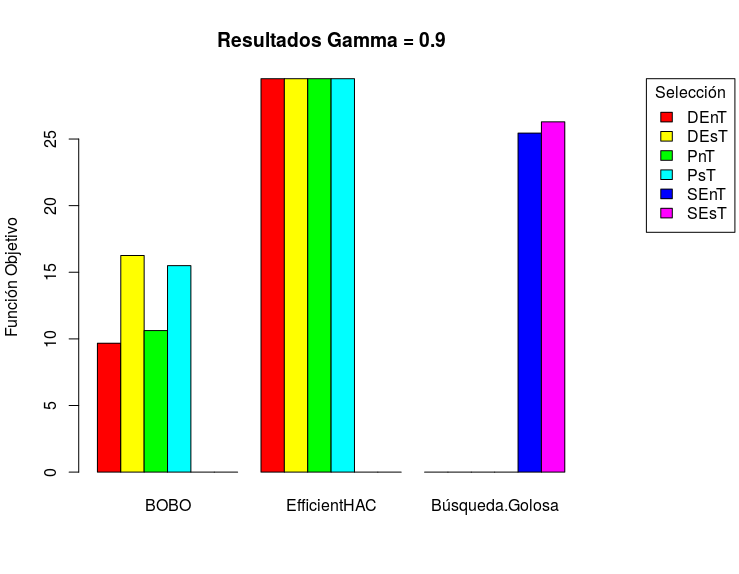
\includegraphics[width=0.8\textwidth]{resultados/cities/Graficos_agrupados/gamma09-cities.png}
  \caption{Función Objetivo $\gamma$ = $0.9$ vs Algoritmos de resolución}
  \label{res:img-cities-agr-gamma09}
\end{figure}

Al igual que en los demás escenarios de ejecuciones el comportamiento fue el esperado y en todas las estrategias usadas para los distintos algoritmos, aplicando la búsqueda Tabú a la solución obtenida encuentra siempre una mejor. También se puede observar que usando la implementación BOBO para valores de $\gamma$ altos es donde mejor funciona la metaheurística y que la búsqueda golosa siempre esta debajo de la solución HAC.\\
Solo se muestran los gráficos y comportamientos para las pruebas realizadas con un solo presupuesto, pero los mismos tuvieron el mismo efecto a medida que se cambiaba ese valor.
